
\section{Server-Client Synchronisation}

\newcommand{\stepOneName}{lockstep}
\newcommand{\stepTwoName}{simple server client}
\newcommand{\stepThreeName}{server client with simulation}

% topology of network(star diagram, what server does, what client does)
\begin{marginfigure}
	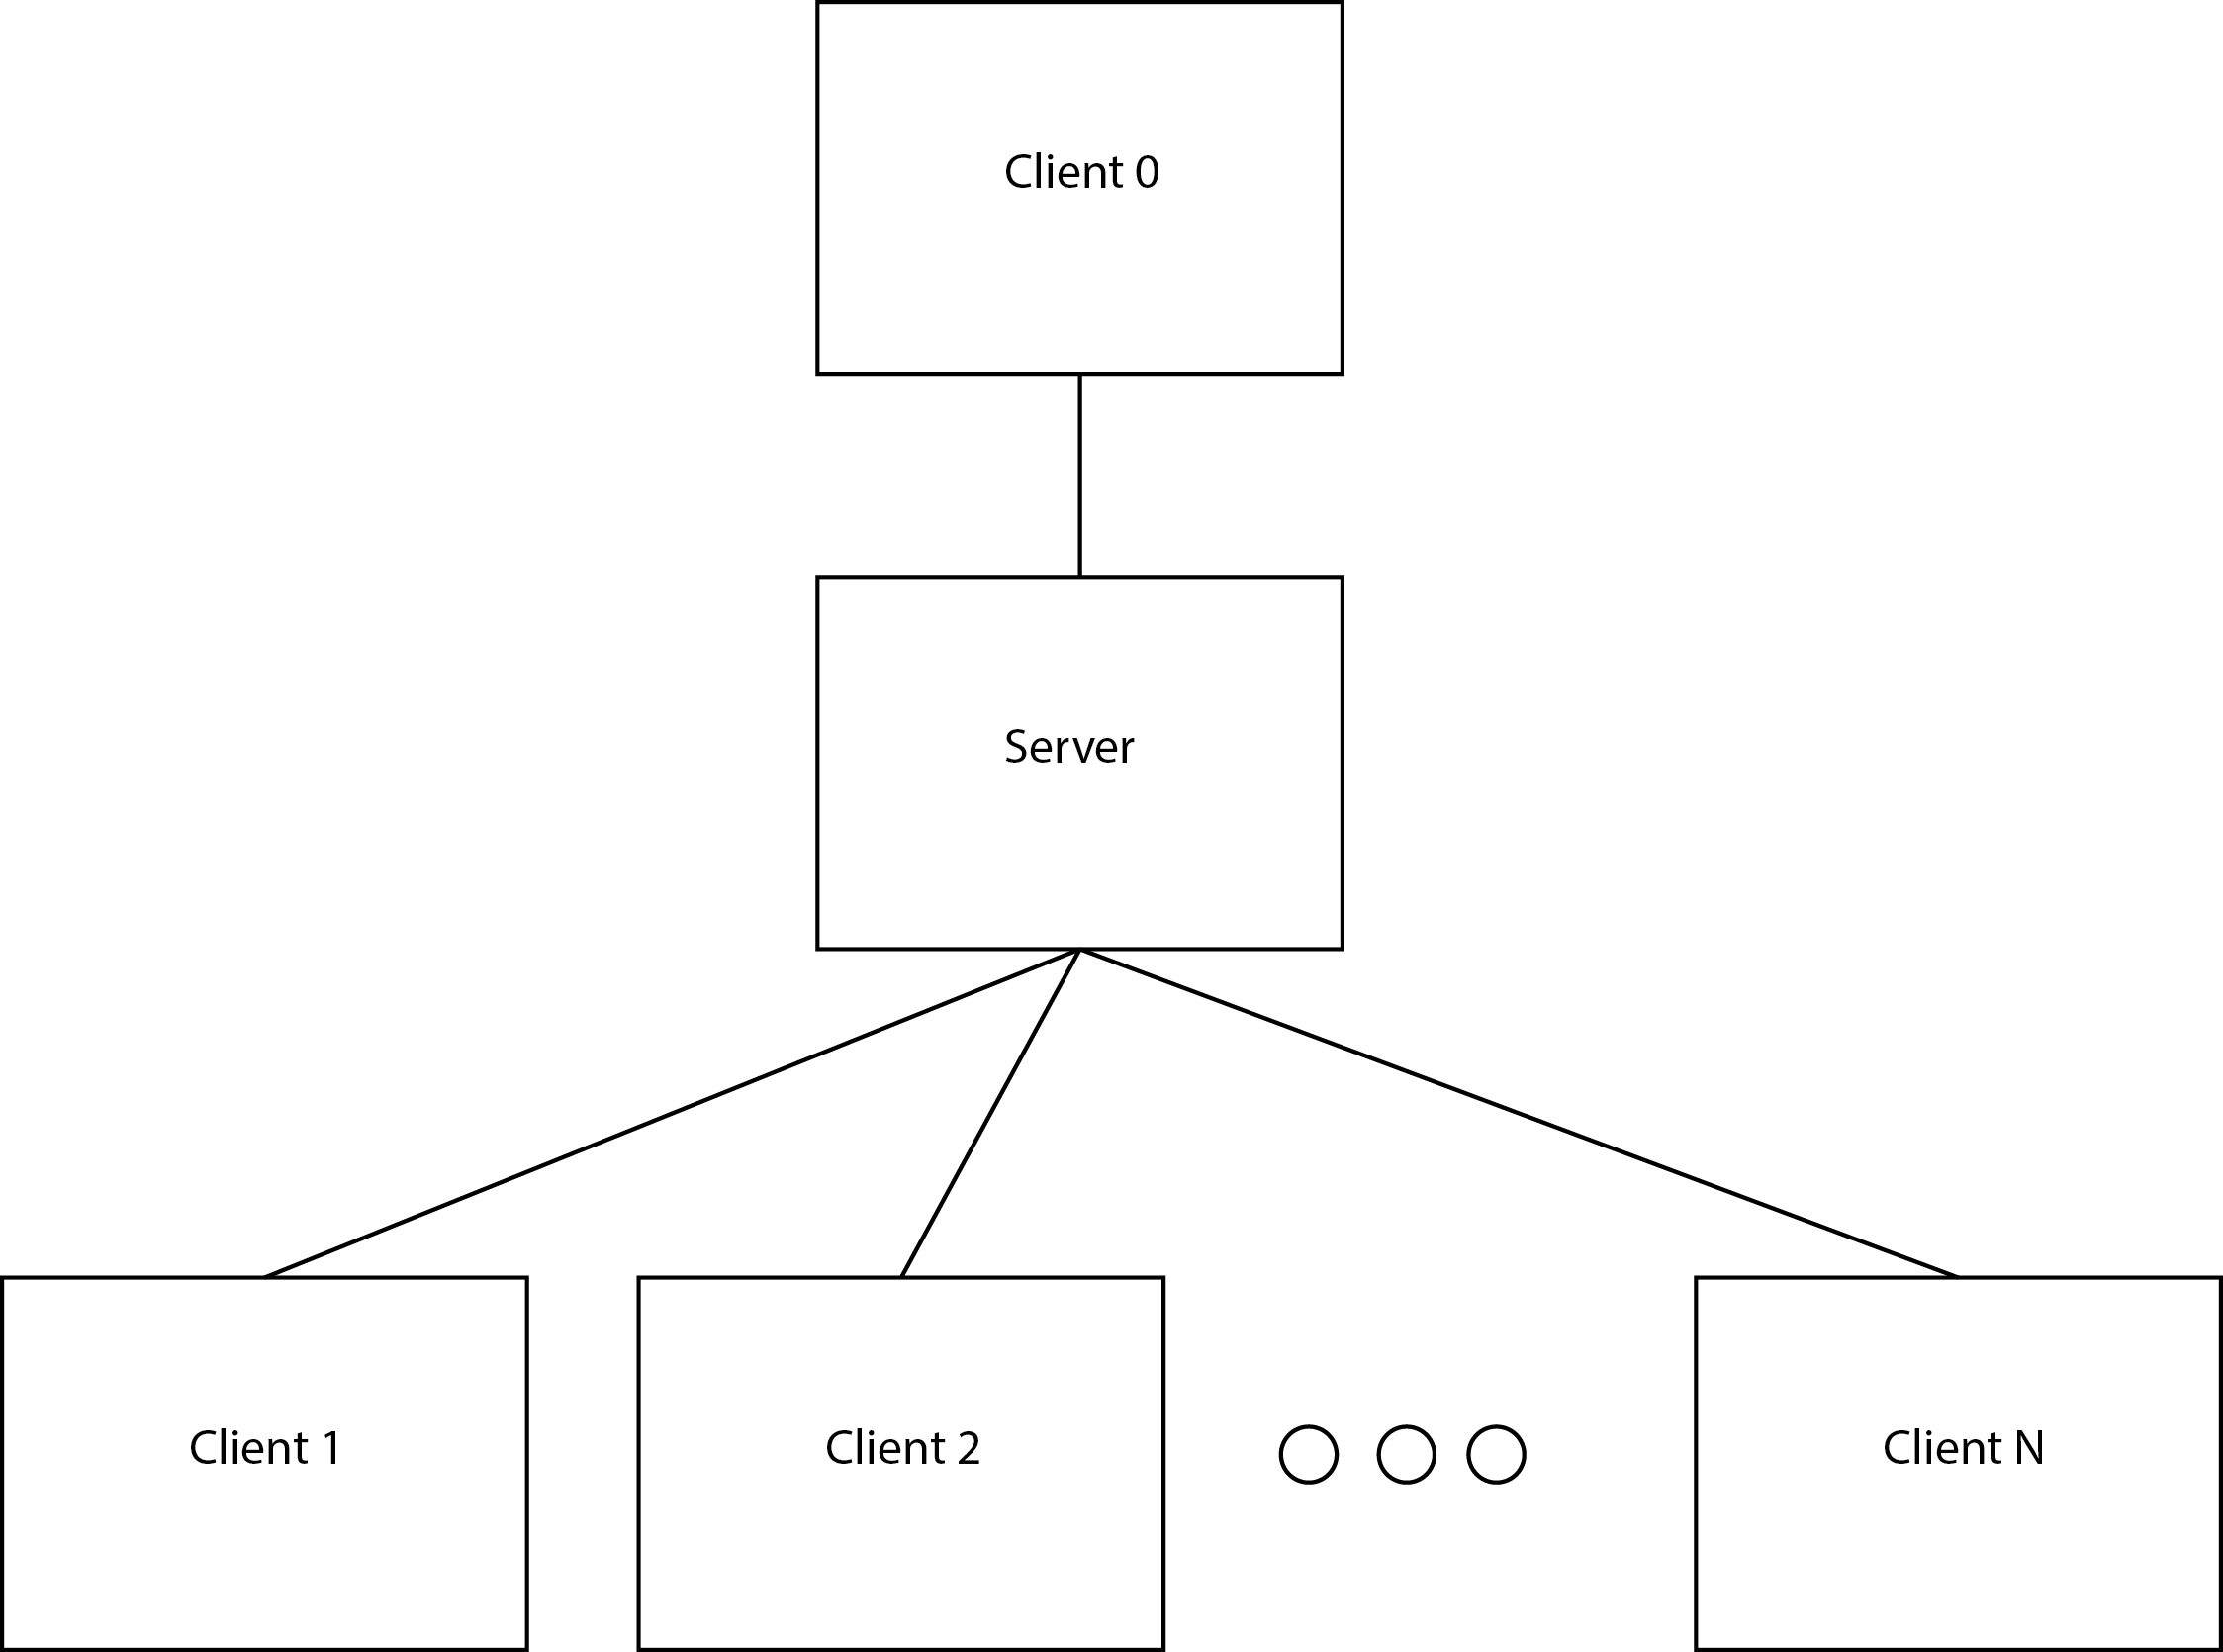
\includegraphics{res/computer_communication_architecture/NetworkTopology.png}
	\caption{
	network topology for multiplayer.
	}
	\label{fig:serverClientSychNetworkTopology}
\end{marginfigure}

The topology is a typical Star Network, with server in centre, and all clients only connecting to server.
There are $N+1$ player connected, where client 0 is the client that is hosting the server.
Since client 0 is hosting the server, they have special permissions to stop the server at any point, ending the game.
This topology greatly simplifies the requirements of the networking, because every client has to only connect to server, and receive all its updates from 1 single place. 

% protocol for synching game states between client server (command, update)
Figure \ref{fig:loops} gives a good representation how the server and a given client communicate.
Both the server and client have a full copy of the model representing the game state.
Their were a variety of benefits from this, the least of which it allowed the clients to scroll around the map without requiring any network traffic.

When the player gives an order, i.e. to move a ship to a given destination, that order is sent to the server in the form of a command.
On the server side, that command is used to 'update' the server's game model. Now the server's game state is at a later version than the clients. The server generates updates that can be applied to all client's game states to bring them to the same version as the server's version.

An example of an update message is: A ship has been given a move order to a location on opposite side of map.
Since their is no simulation on the client side, the ship will only move if the server sends an position update to the clients, moving it slightly closer to its destination. This means that for every time step, every ship that is moving will require an update message send across the network to every client. 

The move update will look something like this:

\begin{margintable}
    \begin{tabular}{l l l l l}
    \toprule
    \emph{shipID} & \emph{x} & \emph{y} & \emph{direction x} & \emph{direction y} \\ 
    \midrule
    43 & 10 & 15 & 0 & 1 \\
    \bottomrule
    \end{tabular}
    	\vspace{1em}
	\caption{example of a position update message}
	\label{tab:positionUpdateExample}
\end{margintable}

Instead of the server telling the client where the ship's destination is, and letting the client move the ship their, the server tells the client when to the next jump location. In the example in Figure \ref{tab:positionUpdateExample} the ship with ID 43 has been given a position update to the new coordinates (10,15), facing North which is (0, 1).

Their are a variety of updates message, depending on which part of the game needs to be updated. 
Originally there was only 3 types of updates:
\begin{description}
\item[addEntity] used for adding an entity to the game. It contains the entity being added to the game.
\item[deleteEntity] used for deleting an entity. An example of use would be when an entity was just blown up. Only contains the entiyID
\item[updateEntity] most common update, used to update an entity. It contains the new entity, and the existing entity is replaced with the entity inside this update.
\end{description}

Having 3 updates provided a very simple design. 
2 out of the 3 updates(addEntity and updateEntity) contains an entity object which is very large in size.
To send an entity object across the network can be very slow and should only be done when necessary.

The addEntity update needs to contain an entity because that entity is currently not in the game, so all the fields of the entity need to be sent across to all the clients. Since addEntity is primarily used at the start of a game when all the entities are loaded into the game, this is not a problem.

However the updateEntity update is sent every time an entity changes location, direction, targets, etc.
Each time an entity's field changes the entire entity must be sent across the network to all the clients.
Not only is this taking up a large amount of bandwidth, but it is sending a large proportion of redundant fields which haven't been changed.
The solution to this was to split the updateEntity update into multiple updates, each one for a common update usage.
The different types of updates to an entity were identifies and a new update message was given to it. 
Table \ref{tab:updateMessageTypes} contains the update messages devised.

\begin{table}
    \begin{tabular}{p{5em} p{15em} p{6em}}
    \toprule
    \emph{Update Type} & \emph{Description} & \emph{Fields} \\
    \midrule
    position & used when both the ship's location and direction has changed & entityID, location, direction \\
    order & when a ship's orders change & entityID, order \\
    goal & when a ship's goal changes & entityID, goal \\
    plan & when a ship's plan to achieve its goal changes & entityID, plan \\
    health & when a ship's hull or shields health changes & entityID, hull health, shield health \\ 
    \bottomrule
    \end{tabular}
    	\vspace{1em}
	\caption{each type of update message, description of its usage, and the fields it will contain}
	\label{tab:updateMessageTypes}
\end{table}

Now, when a ship's field, say direction changes, the direction update message is used instead of the old entity update message.
This is significantly cheaper with regards to network usage because only the ship's ID and new location are sent.

% network traffic calculation
Their were concerns that the volume of traffic required to maintain all the client's game states updates would still be too great for a playable game.
Therefore a traffic analysis was done to estimate how much network traffic would actually be required.
When assumptions are made concerning the game, such as number of ships, number of game steps per second, etc, worst case scenario will be assumed giving the limitations of the game, IE we will know the maximum number of ships the game can have before the game becomes effects by network bandwidth.



The size of each update message will need to be estimated as well as how frequently that message will be sent.

First, the size of field types will need estimating using language independent types such as int, float, double, etc.
This is done in Table \ref{tab:positionUpdateExample}
\begin{margintable}
    \begin{tabular}{p{5em} p{5em}}
    \toprule
    \emph{Field Type} & \emph{Field Size/bytes} \\
    \midrule
    int & 4 \\ 
    long & 8 \\ 
    float & 4 \\
    double & 8 \\    
    \bottomrule
    \end{tabular}
    	\vspace{1em}
	\caption{example of a position update message}
	\label{tab:positionUpdateExample}
\end{margintable}

Now we have estimates of size for the different types, we can assign types to the fields of the message

\begin{margintable}
    \begin{tabular}{p{5em} p{5em} p{5em}}
    \toprule
    \emph{Field Name} & \emph{Size/bytes} \\
    \midrule
    entityID & 4 \\ 
    location & 8 \\
    direction & 8 \\ 
    order & 15 \\
    goal & 9 \\ 
    plan & 100 \\ 
    hull & 4  \\ 
    shield & 4  \\  
    \bottomrule
    \end{tabular}
    	\vspace{1em}
	\caption{example of a position update message}
	\label{tab:positionUpdateExample}
\end{margintable}



For the plan field, it was assumed that each action within the plan was approximately 20 bytes, and that the average plan has 5 steps.

The following table estimates the size of a message to sent across network:
\begin{center}
    \begin{tabular}{| l | l | l |}
    \hline
    Update Type & size / bytes & frequency per game step \\ \hline
    position & 20 & 1 \\ \hline
    order & 19 & 0.2 \\ \hline
    goal & 14 & 0.3 \\ \hline
    plan & 104 & 0.3 \\ \hline
    health & 12 & 0.1 \\ 
    \hline
    \end{tabular}
\end{center}


Now we have the size and frequency of each update message, we can calculate how many bytes are sent to a single client every game step. 
$$ bytes = 20*1 + 19*0.2 + 14*0.3 + 104*0.3 + 12*0.1 $$
$$ bytes = 60.4 $$

We have $S$ representing the number of game steps per second, and $N$ representing the number of clients connected to server.
The number of bytes the server sends per second is
$$ bytes = S * N * 60.4 $$

We now have a formula to calculate network traffic, we need to apply to to various values of $N$ and $S$.

% s=15, 30, 45, 60, n =2, 4, 8, 16
\begin{center}
    \begin{tabular}{| l | l | l |}
    \hline
    S & N & kB/second \\ \hline
    15 & 2 & 1.77 \\ \hline
    \hline
    \end{tabular}
\end{center}

-------------------------- worked upto here ------------------


constants for calculation:
\begin{center}
    \begin{tabular}{| l | l |}
    \hline
    Constant & Value \\ \hline
    world updates / second & 30 \\ \hline
    ships & 40 \\
    \hline
    \end{tabular}
\end{center}

A 

The next step was to calculate the size of a ship update message.

Hence a single ship movement update message would be:
$$ size = (shipID, x, y, directionX, directionY, hullHealth) = 5 * 4 bytes = 20 bytes $$
To send a single ship update to a single client is 20 bytes.



			world updates per second 30
			ships in world = 40
			bullets in world = 1000
			ship movement update = (shipId, x, y, direction) = 4 * 4bytes = 16 bytes.
			bullet movement update = (bulletId, x, y, direction) = 4 * 4bytes = 16bytes
			per client:
				per update:
 					ship data = 40 * 16bytes = 640bytes
					bullet data = 1000 * 16bytes = 16000bytes
					total data = 16640bytes
			    per second = 30 * 16640 = 499200bytes = 487.5KB/S
			3 clients = 3 * 487.5KB/s = 1462.5KB/s = 1.43MB/s

% advantages/disadvantages of lockstep
% advantages/disadvantages of server client with simulation


\begin{comment}

This section talks about how multiplayer was achieved.
This includes the network topology.
server-client allows master copy to exist on server.

- master copy of world on server
- clients perform no logic, only apply updates to
- 




----------------------------------- old gay -----------------------------------------

we need to work out how the computers talked to each other very early on
2 considerations: peer 2 peer, client-server
  - advantages of peer 2 peer
  - advantages of peer server-client
  - why server-client chosen 
  - issues experienced with server-client
    - jumpy ship movements
\end{comment}

The game was designed around being multiplayer, so our first goal was to decide how the player's computers would talk to each other.
Since their was an arbitrary number of players (greater than 1), We needed a system that would scale, but would also be robust.
The game was expecting all players to be on the same LAN (Local Area Network), hence a high bandwidth was available for the communications.

There are 3 strategies for the interactions between computers:
\begin{itemize}
\item \stepOneName
\item \stepTwoName
\item \stepThreeName
\end{itemize}


\begin{marginfigure}
	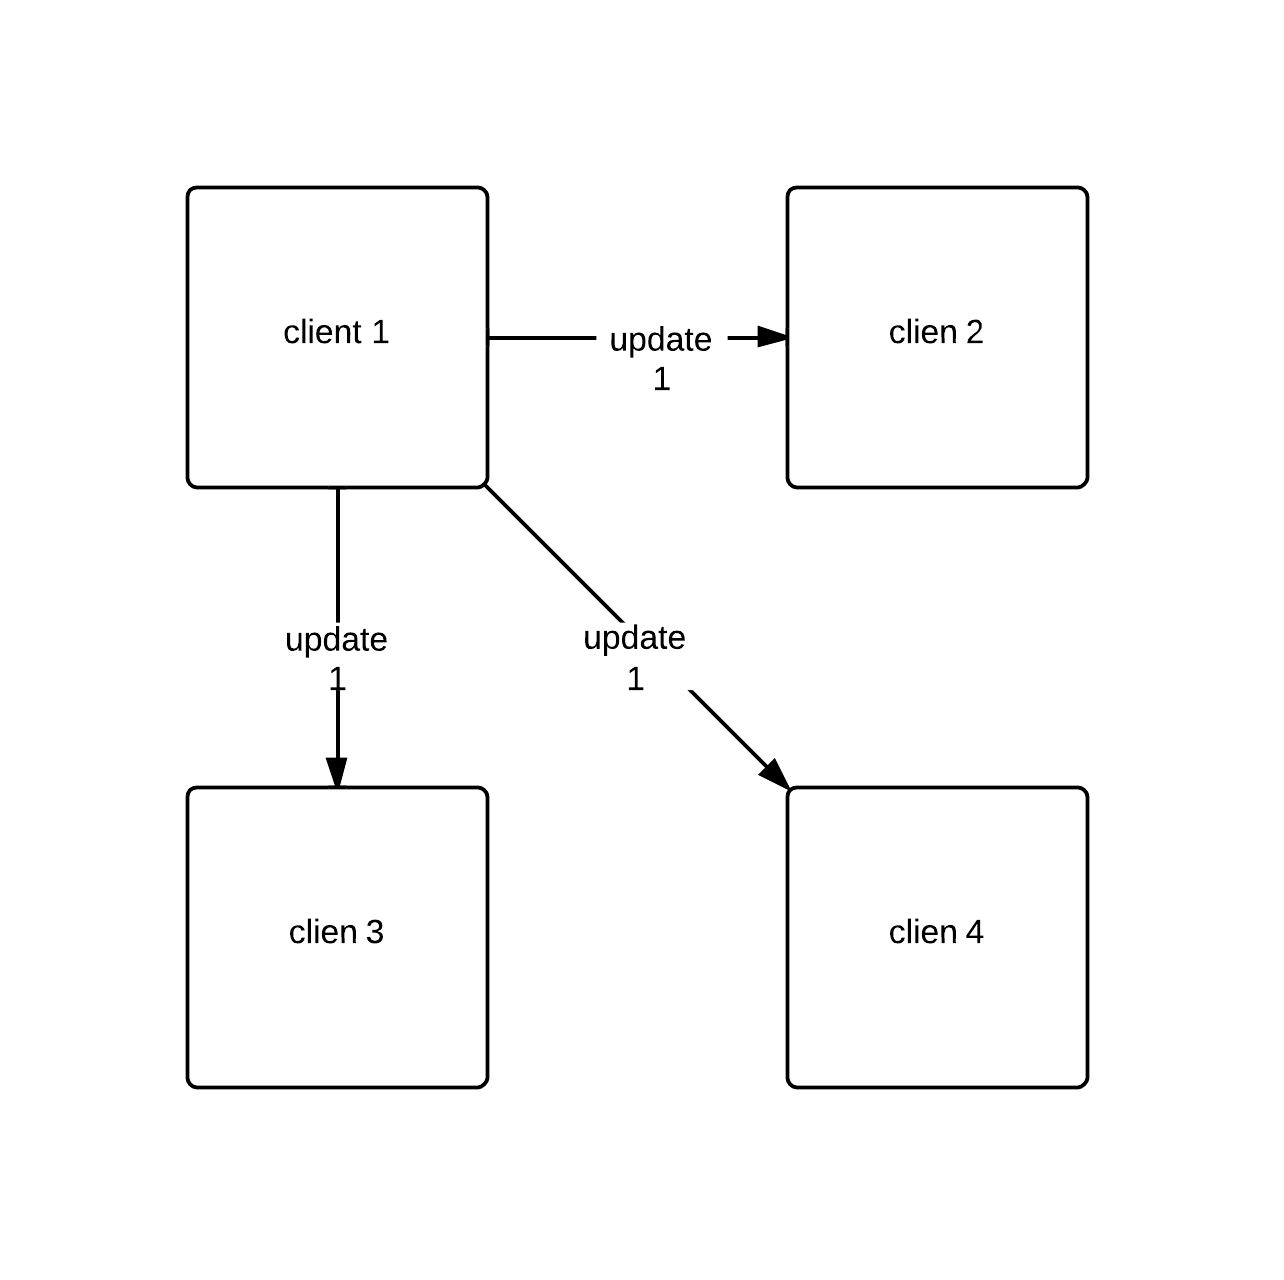
\includegraphics{res/computer_communication_architecture/ServerClientSynchronizationP2P.png}
	\caption{
	\stepOneName : 4 clients connected. client 1 has just modified its game state, so it send the update to all other clients.
	}
	\label{fig:serverClientSychP2P}
\end{marginfigure}

% what
\stepOneName is a peer to peer strategy, in which each computer has a full model of the game. Figure \ref{fig:serverClientSychP2P} shows an example of this strategy. 
Their are 4 computers within game. Each client (client 1, client 2, client 3, and client4) have a full copy of the game.
When client 1 updates performs some actions, they must update their game state, and send this update to all other clients.

\begin{marginfigure}[-30em]
	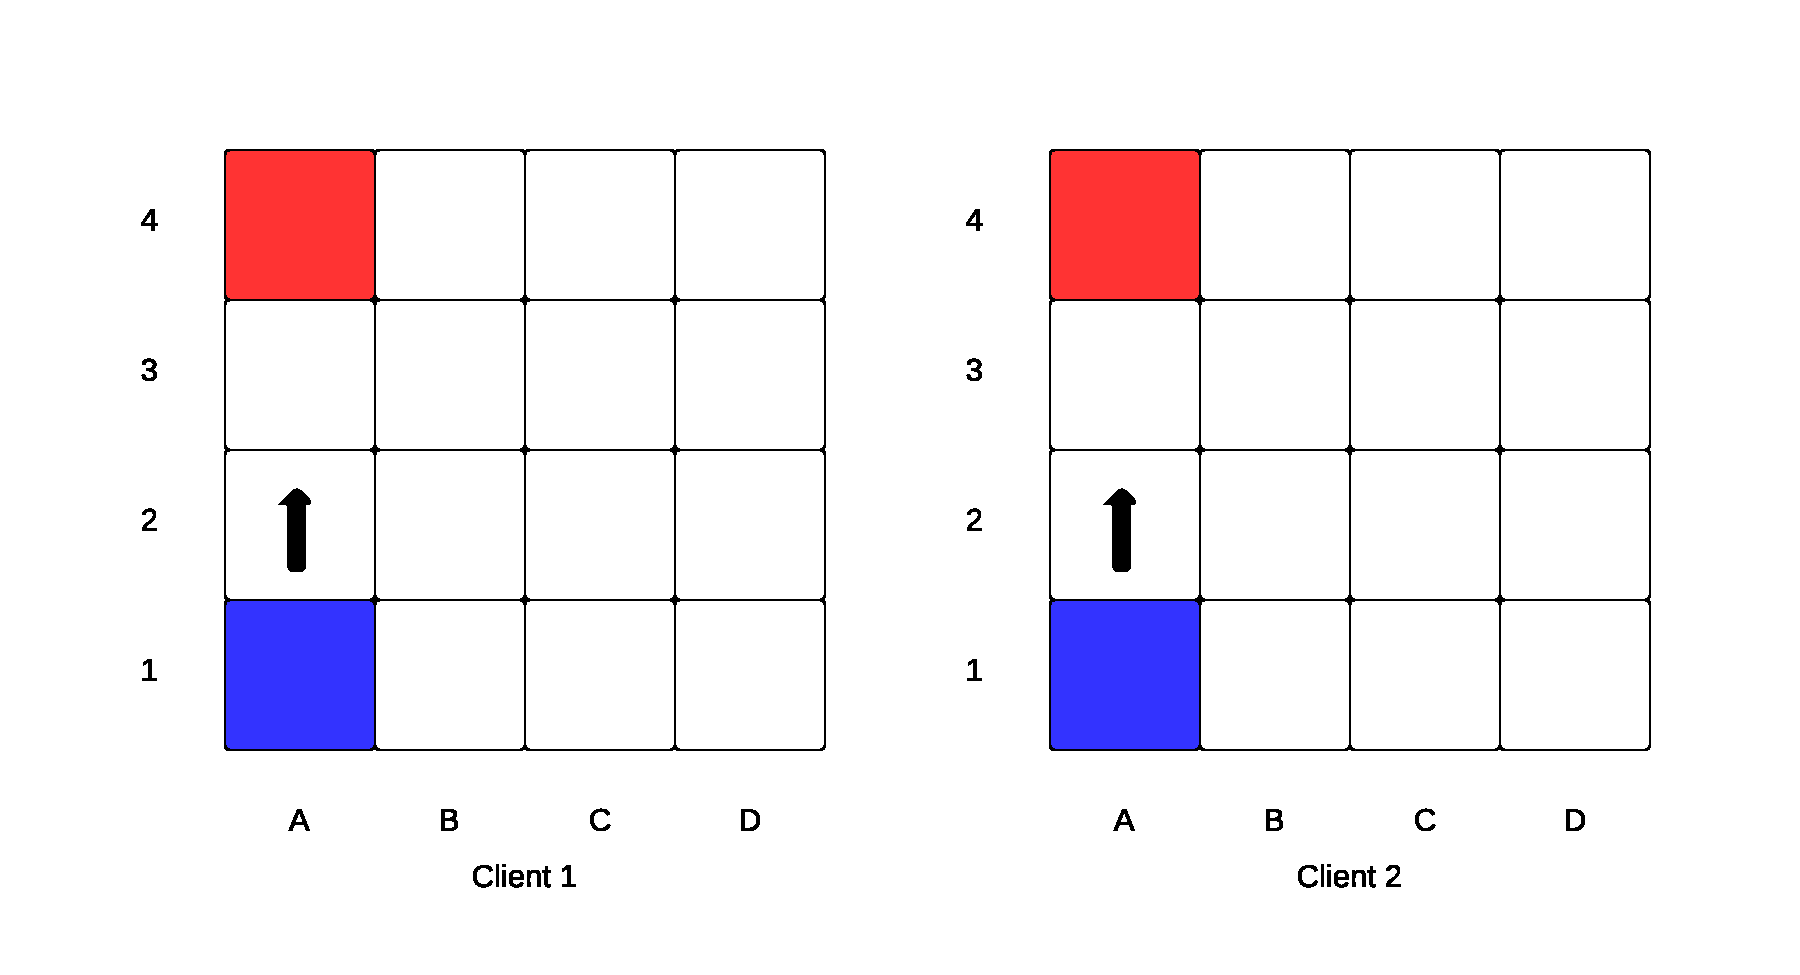
\includegraphics{res/computer_communication_architecture/ServerClientDesynchronisation1.pdf}
	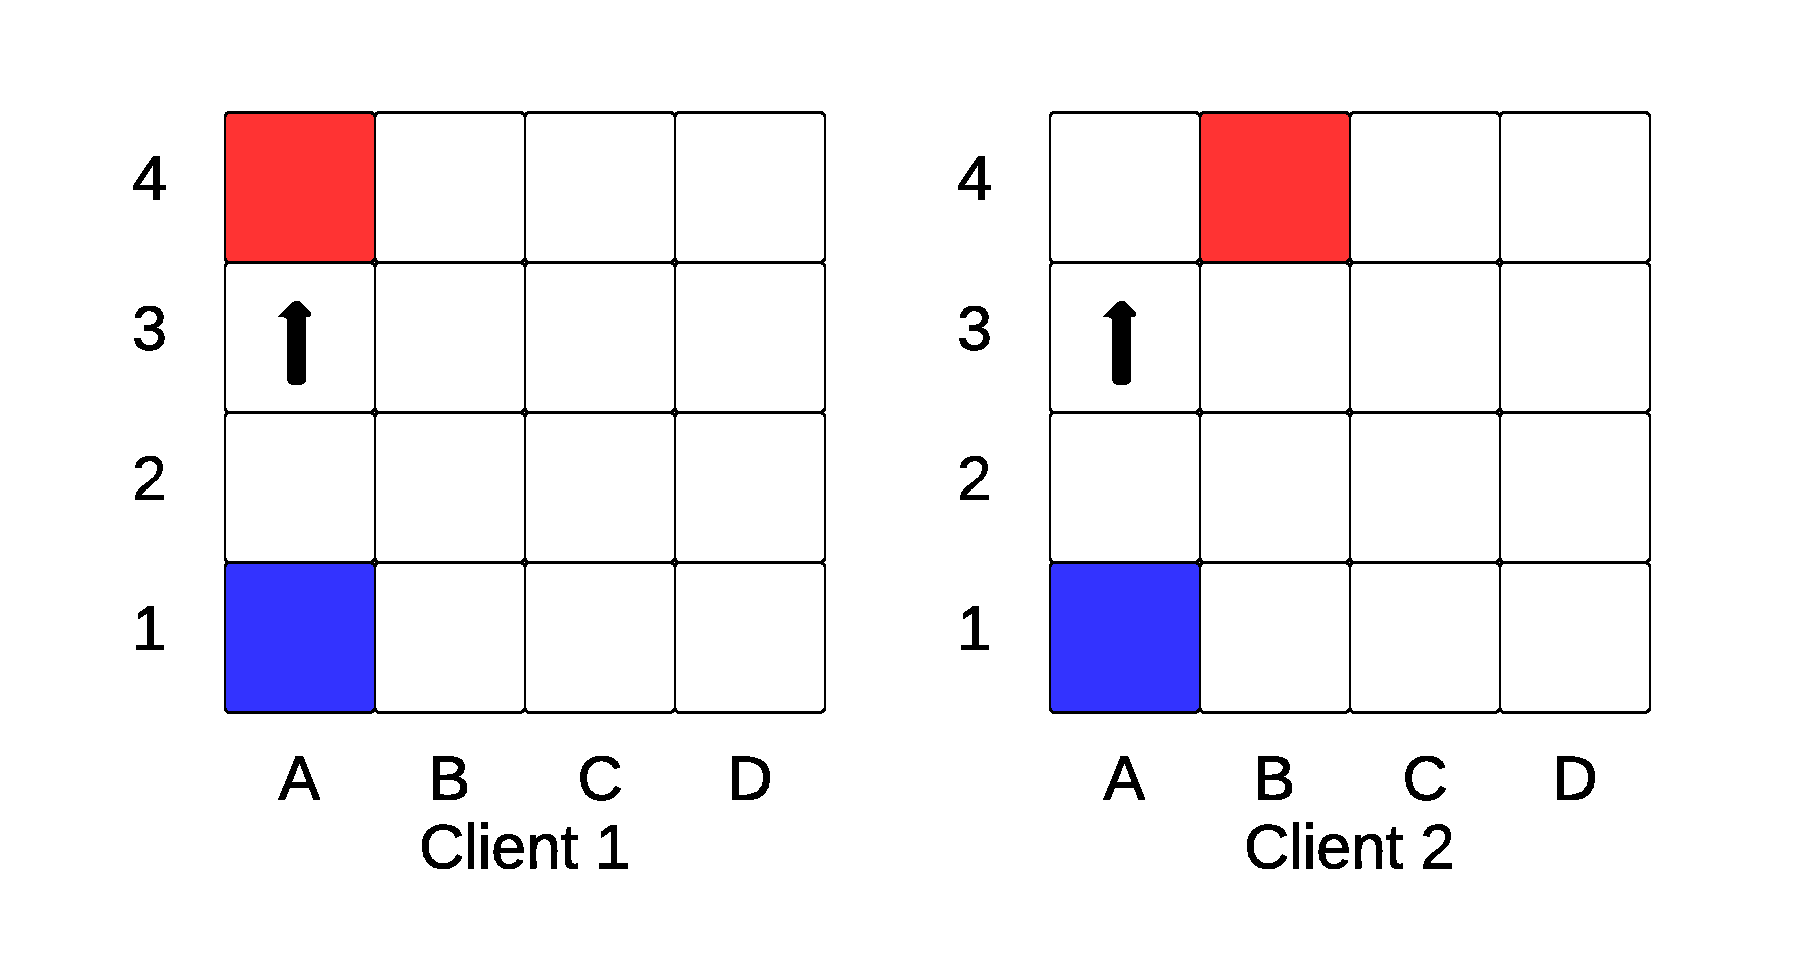
\includegraphics{res/computer_communication_architecture/ServerClientDesynchronisation2.pdf}
	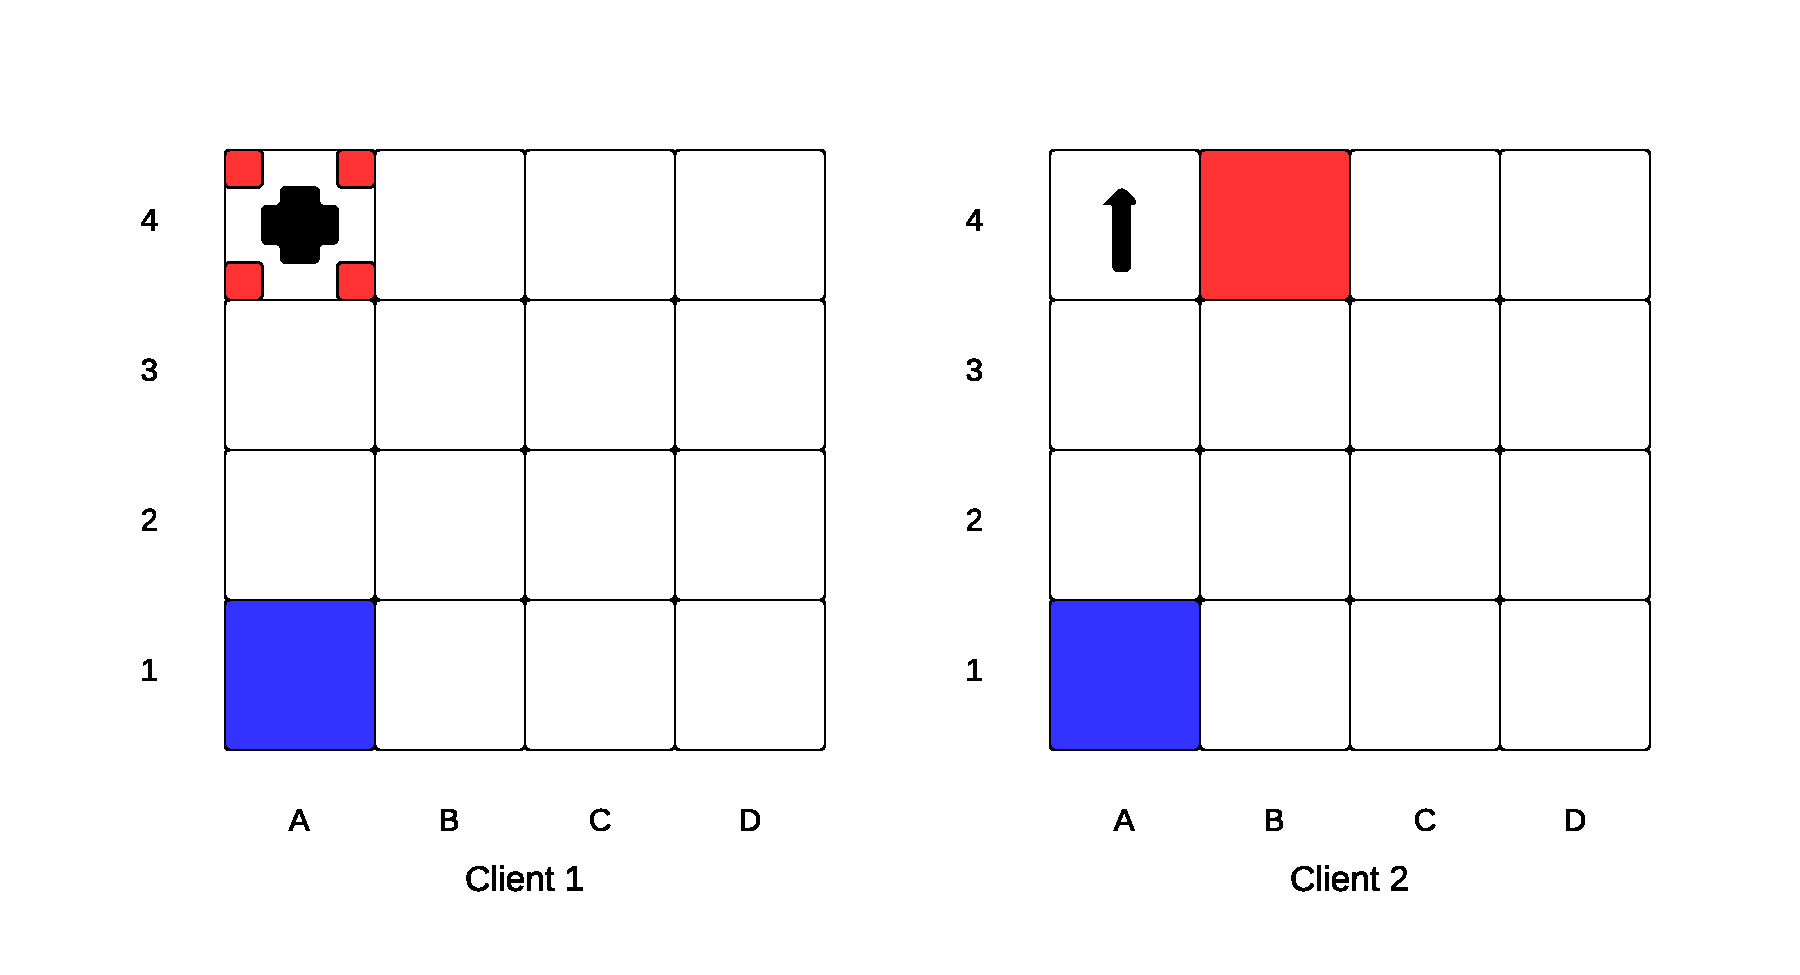
\includegraphics{res/computer_communication_architecture/ServerClientDesynchronisation3.pdf}		
	\caption{
	\stepOneName : example of desynchronization when using the \stepOneName strategy. Client 1 on left, client 2 on right. 
	Each diagram represents state of game for that clients at a given time period.	3 diagrams vertically aligned, First one is top, second one is middle, third one is bottom.
	}
	\label{fig:serverClientDesync}
\end{marginfigure}

% advantages
%   playable with slow networks
This strategy means players can continue to play games on networks with high latency, without any lag. When packets are delayed, the client can continue to play the game, and the game is updated when the packet arrives.
%   no dedicated server required
No client is picked to act as server, which causes game to end if that selected client disconnects.
Since all clients act as server, any client can disconnect and the game continues, providing more robustness which is highly desirable for games with long game intervals, such as Civilization series\cite{civilizationInMyPants}.



% disadvantages
%   disynchronization
Maintaining synchronisation when using a peer-2-peer protocol can be very challenging from a technical point of view, with non-determinism being caused by messages being received by clients at different times causing race conditions.
When this happens in a game, it can cause clients game states to desynchronise.
For example, In Figure \ref{fig:serverClientDesync}, there are 2 clients.
%   corrupted client can effect the entire game



% res/computer_communication_architecture




% lockstep
%   - each client has the master copy of the world
%   - when a client does something, it tells all others
%   - problems:
%     - desycnhronization
%     - currupted client fucks up everyone

% simple server client
%   - it's what we've implemented
%   - no simulation on clients
%   - 1 server that has master copy
%   - server does all processing and sends updates to clients
%   - clients just render the world and send commands to server

% server client with simulation
%   - similar to simple server client but client does 'some' simulation. They in no way can effect the world.
%   - for instance if client knows ships destination and current location it can render the ship graciously moving instead of jumping on every update.

